% ============================================================================
% ViLatent -- ACIIDS 2027 submission (Springer LNCS/LNAI, single column).
%
% Venue constraints (aciids.pwr.edu.pl/2027/submit.html, read 2026-10-23):
%   * full paper 12--15 pages INCLUDING figures, tables and references; more pages
%     may incur extra charges. Check with `python check_pages.py` after building.
%   * Springer LNCS/LNAI template, PDF through EasyChair, English only.
%   * deadline 31 October 2026 (extended), 23:59 AoE.
%   * author names stay in the PDF (single-blind; the author list cannot change
%     once reviewing starts).
%   * similarity screening includes SELF-plagiarism: do not paste text from the
%     LACC or ViWord-C papers.
%
% Placeholders (see README.md):
%   \tbd       a result that does not exist yet (red "??.?")
%   \prelim{x} a measured number that must be re-checked on the final setting (blue)
%   \todo{...} a short note to the authors (red, draft only)
% \draftfalse turns all three into compile errors, so a submission cannot keep one.
% ============================================================================
\documentclass[runningheads,a4paper]{llncs}

% T5 for the Vietnamese examples (prompt, answers); the running text is T1. vntex needs
% `nocaptions`, otherwise it renames the captions to Vietnamese ("Hình", "Bảng").
\usepackage[T5,T1]{fontenc}
\usepackage[utf8]{inputenc}
\usepackage[nocaptions]{vntex}
\usepackage{graphicx}
\usepackage{booktabs}
\usepackage{amsmath,amssymb}
\usepackage{cite}            % numeric citations sorted and compressed: [2,5,7]
\usepackage{xcolor}
\usepackage{tikz}
\usepackage{pgfplots}        % Figures 2 and 3 (figures/curves.tex, written by scripts/paper_figures.py)
\pgfplotsset{compat=1.17}
\usetikzlibrary{positioning,arrows.meta,fit,calc}
\usepackage[hidelinks]{hyperref}
\renewcommand\UrlFont{\color{blue}\rmfamily}
\urlstyle{rm}

\newif\ifdraft
\drafttrue   % \draftfalse before submitting: every leftover placeholder becomes an error
\newcommand{\tbd}{\ifdraft\textcolor{red}{??.?}\else
  \PackageError{main}{a result placeholder (\string\tbd) is left}{Fill it from results/}\fi}
\newcommand{\prelim}[1]{\ifdraft\textcolor{blue}{#1}\else
  \PackageError{main}{a preliminary number (\string\prelim) is left}{Re-check it, then remove the macro}\fi}
\newcommand{\todo}[1]{\ifdraft{\color{red}\footnotesize[TODO: #1]}\else
  \PackageError{main}{a TODO note is left}{Resolve it}\fi}

\newcommand{\mem}{\ensuremath{\langle\mathrm{mem}\rangle}}
\newcommand{\cmem}{\ensuremath{\langle/\mathrm{mem}\rangle}}
\newcommand{\viet}[1]{\textit{#1}}

\begin{document}

\title{ViLatent: Soft Context Compression with Question-Aware Evidence for a Frozen Vietnamese Reader}
\titlerunning{ViLatent: Soft Context Compression for a Frozen Vietnamese Reader}

% First author: ORCID 0009-0007-7623-2413 (public record: given names "Ngoc Thien", family name
% "Than", Hanoi University of Industry; read 2026-10-23).
% Names are written given names first, family name last, as in the ORCID records, so that Springer
% indexes the family name correctly (decided 2026-10-23; the LACC paper used "Thân Ngọc Thiện").
% TODO(authors): co-author names, affiliations, e-mails and ORCID iDs. The list cannot change
% after reviewing starts.
\author{Ngoc Thien Than\inst{1}\orcidID{0009-0007-7623-2413} \and
Co-Author Name\inst{1}\orcidID{0000-0000-0000-0000}}
\authorrunning{N. T. Than et al.}
\institute{School of Information and Communication Technology,\\
Hanoi University of Industry, Hanoi, Vietnam\\
\email{thien.than@haui.edu.vn}, \email{coauthor@haui.edu.vn}}

\maketitle

% Abstract: 150--250 words. The result sentences are written for the outcome the pre-specified
% rule decides; if it fails, rewrite them as a controlled finding (README.md, "Two outcomes").
\begin{abstract}
Soft context compression lets a frozen large language model (LLM) read a document as a few learned vectors instead of its tokens.
We ask when such a memory is worth more than text under the same reader-token budget, for Vietnamese, where soft compression has not been studied.
ViLatent writes a question-blind memory with a writer copied from the reader's bottom layers; a single multi-rate writer serves every compression ratio.
At reading time, sentences selected by BM25 for the question fill the rest of the budget, and a three-stage cascade reads more text only when the answer is not found verbatim in the evidence or the reader is unsure.
With the Qwen3.5-2B reader, we compare ViLatent with truncation, lead sentences, LLMLingua-2, BM25 and a trained PhoBERT sentence selector at 4$\times$, 8$\times$ and 16$\times$, on single UIT-ViQuAD~2.0 passages and on ViQuAD-Long, which joins all passages of an article, using article-disjoint splits, a pre-specified decision rule and a single test run.
On ViQuAD-Long at 4$\times$, ViLatent reaches \tbd{} F1 against \tbd{} for the best hard compressor (difference \tbd{}, 95\% CI [\tbd{}, \tbd{}]), and across ratios its advantage over text \tbd{} as the budget shrinks.
A learned context-free prompt with the same evidence and memory swapped from another article separate memory content from learned answer style.
Query-blind writing costs \tbd{} F1 against a writer that sees the question, and the cascade keeps \tbd\% of full-context F1 with \tbd{} reader tokens per question.
We release code, checkpoints and splits.

\keywords{Context compression \and Soft prompts \and Large language models \and Vietnamese \and Question answering \and Long documents}
\end{abstract}

\section{Introduction}
\label{sec:intro}

Context compression lowers the cost of reading a document with a large language model (LLM), here called the \emph{reader}, by shortening what it has to process; the saving adds up when the same document is queried many times.
\emph{Hard} compressors keep part of the original text, either tokens scored by a small model~\cite{jiang2023llmlingua,pan2024llmlingua2} or text chosen for the question~\cite{jiang2024longllmlingua}.
\emph{Soft} compressors encode the context into continuous vectors that the reader consumes through its input embeddings~\cite{mu2023gist,ge2024icae,cheng2024xrag,li2024_500x}; recent designs keep the reader frozen and train only a small encoder, the \emph{writer}, by distilling the answers the same reader gives with the full context~\cite{xu2026latentpress,liu2025sac,rahman2026cmc}.

The two families fail differently.
A selected sentence reaches the reader verbatim, with its numbers and names intact, but whatever is not selected is lost.
A soft memory touches every part of the document, but blurs it: for one soft compressor, only about a quarter of dates and cardinal numbers survive in text reconstructed from its memory~\cite{lajewska2025information}.
Which loss hurts more should depend on the budget and on the document: when the budget is generous or the document short, a good selector may already include the answer, whereas a tight budget over a long document leaves text selection little room.
We therefore ask \emph{when soft memory is more worthwhile than text under the same reader-token budget}, rather than whether one family wins everywhere.
We study the question for Vietnamese: to our knowledge no soft compressor has been reported for it, and for extractive compressors results do not carry over evenly across languages~\cite{lukauskas2026lost}; we treat language as a coverage gap and do not test whether Vietnamese itself makes compression harder.

A writer that ignores the question makes the memory reusable, since caches compressed for one query lose quality when reused for others~\cite{kim2025kvzip}, but it may drop the detail a later question needs.
Writers that see the question~\cite{cao2024qgc,louis2025oscar} avoid this loss but give up reuse; trained under identical conditions, a query-aware compressor beats its query-agnostic counterpart by up to 5.7 points~\cite{sakhno2026adamem}.
Systems that read a gist and then return to the original text keep reuse and recover most of the loss~\cite{lee2024readagent,xie2026lensvlm}, and routing uncertain questions to the full context keeps quality close to full reading at lower cost~\cite{li2024selfroute}.

ViLatent combines these observations for a frozen Vietnamese reader: \emph{write once, read with the question}.
A writer built from the reader's bottom layers compresses each document once, without the question; since its states do not depend on the pooling ratio, one multi-rate writer serves every ratio and every split of the budget.
When a question arrives, BM25~\cite{robertson2009bm25} selects original sentences, and memory and sentences share one reader-token budget, the same budget every hard baseline receives.
A three-stage cascade then reads more text only when needed: it accepts the answer if it appears verbatim in the evidence and the reader is confident, otherwise it reads a larger BM25 selection, and as a last resort the full document.

A trained compressor compared with untrained baselines can win for the wrong reasons, and the evaluation guards against three of them.
(i)~\emph{Leakage.} UIT-ViQuAD passages come from Wikipedia articles~\cite{nguyen2020viquad,nguyen2022vlsp}; in our earlier passage-level split, 81\% of the training questions came from the articles of the dev passages, so all held-out sets are now split by article.
(ii)~\emph{Answer style.} ViLatent learns from gold answers while most hard baselines are zero-shot; a learned context-free prompt with the same evidence and training, a memory swapped from another article, and a trained hard selector bound this effect.
(iii)~\emph{Budget.} Memory vectors count like text tokens, and the free parameters of the hard baselines are tuned on the selection split.
% TODO(authors): cite the LACC paper here if it is published or under review and citable
% ("hard compression reached a ceiling in our earlier study"); do not reuse its text.

We ask three questions.
\textbf{RQ1:} at equal budget, does ViLatent-ME beat hard compression on long documents (ViQuAD-Long) and single passages at 4$\times$, 8$\times$ and 16$\times$, and does its advantage come from the memory content rather than from learned answer style?
\textbf{RQ2:} what does query-blind writing cost against a writer that sees the question?
\textbf{RQ3:} how many reader tokens does a cascade need to retain 95\% of full-context F1?
Our contributions are:
\begin{itemize}
\item ViLatent, to our knowledge the first soft compressor for a frozen Vietnamese reader and for a reader that mixes Gated DeltaNet~\cite{yang2025gdn} and attention layers, Qwen3.5~\cite{qwen35}, with a \emph{multi-rate} writer: one checkpoint for all compression ratios and memory shares (Sect.~\ref{sec:method}).
\item ViQuAD-Long, an article-level version of UIT-ViQuAD~2.0, and a controlled soft-versus-hard comparison across ratios with article-disjoint splits, a pre-specified decision rule and answer-style controls (Sect.~\ref{sec:setup}).
\item A cascade with an answer-in-evidence check, and end-to-end cost accounting that includes the writer: latency and the number of questions per document at which writing pays off (Sect.~\ref{sec:results}).
\item Code, checkpoints and splits.\todo{repository URL}
\end{itemize}
% Findings, one sentence per RQ, filled from results/ after the test run. If the rule fails (outcome B,
% README.md item 3), say which condition failed and what the controls show.
On ViQuAD-Long test at 4$\times$, ViLatent-ME reaches \tbd{} F1 against \tbd{} for the best hard compressor (95\% CI of the difference [\tbd, \tbd]) and \tbd{} for the learned prompt with the same evidence, and the gap \tbd{} from 4$\times$ to 16$\times$ (RQ1); seeing the question changes F1 by \tbd{} (RQ2); the cascade keeps 95\% of full-context F1 at \tbd{} tokens per question (RQ3).

\section{Related Work}
\label{sec:related}
% Descriptions and numbers are checked against the sources in notes/references_verified.md.

\paragraph{Hard compression.}
Hard compressors keep the input human-readable and need no access to the reader's weights.
LLMLingua prunes tokens by the perplexity of a small model under a budget controller~\cite{jiang2023llmlingua}, LongLLMLingua makes this question-aware~\cite{jiang2024longllmlingua}, and LLMLingua-2 casts compression as keep-or-drop token classification with a multilingual encoder~\cite{pan2024llmlingua2}.
Hard selection is both a competitor and a part of ViLatent, whose evidence is a question-aware sentence selection.

\paragraph{Soft compression.}
Gist tokens compress a prompt through modified attention masks~\cite{mu2023gist}; ICAE trains a LoRA-adapted copy of the LLM to produce memory slots with autoencoding and language-modelling objectives~\cite{ge2024icae}; 500xCompressor passes compressed tokens as key--value pairs~\cite{li2024_500x}; xRAG maps one retriever embedding to a single input token~\cite{cheng2024xrag}.
Recent writers keep the reader frozen and learn from its own answers: SAC drops the autoencoding objective~\cite{liu2025sac}, CMC trains a separate encoder with answer-aligned losses~\cite{rahman2026cmc}, and LatentPress, the cheapest of them and the basis of ViLatent, copies the reader's bottom layers, mean-pools their states and maps them through a linear adapter initialised to the identity, trained with cross-entropy and a KL term towards the full-context reader~\cite{xu2026latentpress}.
None of these works reports results for Vietnamese.

\paragraph{The question during compression.}
Query-guided compressors condition the encoder on the question~\cite{cao2024qgc,louis2025oscar}, which prevents reuse; AdaMem retrains a query-agnostic and a query-aware compressor with the same data and finds the query-aware one better by 3.9 (NQ) and 5.7 (HotpotQA) points at 16$\times$~\cite{sakhno2026adamem}, while KVzip shows that a cache pruned for one query loses quality on others~\cite{kim2025kvzip}.
Other systems keep a query-blind memory and use the question only when reading: ReadAgent looks up original pages from a gist memory~\cite{lee2024readagent}, SeDeM decompresses selected blocks of a hidden-state memory~\cite{haghifam2026sedem}, LensVLM expands selected pages of a compressed visual context back to text~\cite{xie2026lensvlm}, and Self-Route falls back to the full context when the reader declares a cheap one insufficient~\cite{li2024selfroute}.
An analysis of information preservation finds that xRAG keeps only 22\% of dates and 26\% of cardinal numbers and suggests keeping such details as hard tokens next to a soft prompt~\cite{lajewska2025information}, which is what the evidence sentences of ViLatent do.
ViLatent applies ``write blind, read with the question'' to a frozen reader in a language these studies do not cover, and asks at which budgets the memory is worth its positions.

\section{ViLatent}
\label{sec:method}

ViLatent trains only a writer and its adapter, never the reader (Fig.~\ref{fig:overview}).

% Figure 1: ViLatent-ME and the MEF fallback. Trainable blocks are blue; the reader is frozen.
% Absolute coordinates in mm; the drawing is 115 mm wide (LNCS text width: 122 mm).
\begin{figure}[t]
\centering
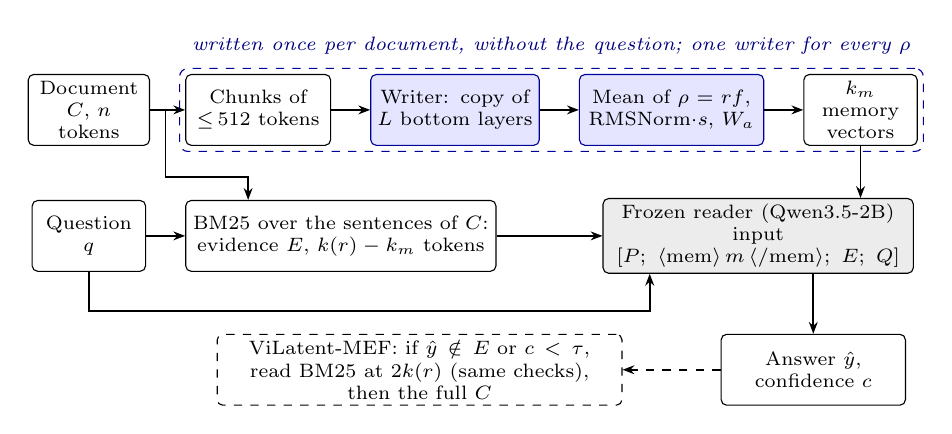
\begin{tikzpicture}[x=1mm, y=1mm, font=\scriptsize,
  box/.style={draw, rounded corners=2pt, align=center, minimum height=9mm, inner sep=2pt},
  train/.style={box, fill=blue!10, draw=blue!60!black},
  frozen/.style={box, fill=gray!15},
  arr/.style={-{Stealth[length=1.5mm]}, semithick}]
  % writing: once per document, without the question
  \node[box, text width=14mm] (ctx) at (8,0) {Document\\$C$, $n$ tokens};
  \node[box, text width=17mm] (chunk) at (29.5,0) {Chunks of\\$\le$\,512 tokens};
  \node[train, text width=20mm] (writer) at (54.5,0) {Writer: copy of\\$L$ bottom layers};
  \node[train, text width=22mm] (pool) at (82,0) {Mean of $\rho = rf$,\\RMSNorm$\cdot s$, $W_a$};
  \node[box, text width=13mm] (memory) at (106,0) {$k_m$ memory\\vectors};
  \draw[arr] (ctx) -- (chunk);
  \draw[arr] (chunk) -- (writer);
  \draw[arr] (writer) -- (pool);
  \draw[arr] (pool) -- (memory);
  \node[fit=(chunk)(writer)(pool)(memory), draw=blue!60!black, dashed, rounded corners=3pt, inner sep=2pt,
        label={[font=\scriptsize\itshape, text=blue!50!black, yshift=0.5mm]above:written once per document, without the question; one writer for every $\rho$}] {};
  % reading: the question chooses the evidence
  \node[box, text width=13mm] (q) at (8,-16) {Question $q$};
  \node[box, text width=38mm] (bm25) at (40,-16) {BM25 over the sentences of $C$:\\evidence $E$, $k(r) - k_m$ tokens};
  \node[frozen, text width=38mm] (reader) at (93,-16) {Frozen reader (Qwen3.5-2B)\\input $[P;\ \mem\, m\, \cmem;\ E;\ Q]$};
  \draw[arr] (q) -- (bm25);
  \draw[arr] (bm25) -- (reader);
  \draw[arr] (17.75,0) -- (17.75,-8.5) -| ($(bm25.north west)+(8,0)$);
  \draw[arr] (memory.south) -- (memory.south |- reader.north);
  \draw[arr] (q.south) -- ++(0,-5) -| ($(reader.south west)+(6,0)$);
  % answer and fallback
  \node[box, text width=22mm] (ans) at (100,-33) {Answer $\hat y$,\\confidence $c$};
  \node[box, dashed, text width=50mm] (full) at (50,-33) {ViLatent-MEF: if $\hat y \notin E$ or $c < \tau$,\\read BM25 at $2k(r)$ (same checks),\\then the full $C$};
  \draw[arr] (reader.south -| ans.north) -- (ans.north);
  \draw[arr, dashed] (ans) -- (full);
\end{tikzpicture}
\caption{ViLatent-ME at a budget ratio $r$. The writer and the adapter (blue) are trained; the reader is frozen.
The memory ($k_m = k(rf)$ vectors) and the BM25 evidence share the budget $k(r)$ of Eq.~\eqref{eq:budget}.
ViLatent-MEF reads more text when the answer is not in the evidence $E$ or its confidence is below $\tau$.}
\label{fig:overview}
\end{figure}


\subsection{Reader-Token Budget}
\label{sec:budget}
Every method, soft or hard, reads a document within the same reader-token budget $k(r)$, computed by one function for training, evaluation and every baseline (safeguard~(iii) in Sect.~\ref{sec:intro}).
A document $C$ of $n$ reader tokens, a passage or a whole article, is cut into chunks $c_1,\dots,c_m$ of at most 512 tokens that end at sentence boundaries, with sentences packed greedily.
For a compression ratio $r$, the budget is
\begin{equation}
k(r) = \sum_{i=1}^{m} \left\lceil n_i / r \right\rceil, \qquad n_i = |c_i| .
\label{eq:budget}
\end{equation}
A hard compressor receives a text of at most $k(r)$ reader tokens, counted as the text sits in the prompt; ViLatent receives at most $k(r)$ input positions, vectors and text tokens together.
The two learned boundary embeddings \mem{} and \cmem{} are not counted, just as the label that introduces the passage in a text prompt is not.

\subsection{Multi-Rate Writer}
\label{sec:writer}
The writer is a trainable copy of the reader's bottom $L = 4$ decoder layers.
Unlike LatentPress, which trains only the head on top of the copied layers~\cite{xu2026latentpress}, ViLatent trains these layers too, at a lower learning rate.
In Qwen3.5, layers come in groups of three Gated DeltaNet layers~\cite{yang2025gdn} and one gated attention layer, so $L = 4$ is the shallowest writer with an attention layer.
Chunks are encoded independently, each preceded by a fixed sink token whose state is discarded, because the first position of a sequence can carry very large activations.
Let $h_1,\dots,h_{n_i}$ be the output states of chunk $c_i$ and $G_j$ the $j$-th group of $\rho$ consecutive positions (the last group may be shorter).
The $j$-th memory vector is
\begin{equation}
m_{ij} = W_a \, \Big( s \cdot \mathrm{RMSNorm}\big(\tfrac{1}{|G_j|} \textstyle\sum_{t \in G_j} h_t \big) \Big),
\label{eq:pool}
\end{equation}
where $W_a \in \mathbb{R}^{d \times d}$ starts as the identity and the scalar $s$ starts at the value that gives memory vectors the mean $\ell_2$ norm of the reader's input embeddings.
The states $h_t$ do not depend on the pooling ratio $\rho$, so one writer can pool at any ratio: we train a single writer with $\rho$ drawn for every example, and $W_a$ and $s$ are shared by all ratios.
The writer layers, $s$, $W_a$ and the boundary embeddings (initialised from the embeddings of ``\guillemotleft'' and ``\guillemotright'') are trained; for Qwen3.5-2B ($d=2048$) the adapter alone has 4.19M parameters.
The memory replaces the document text in the reader input:
\begin{equation}
x = \big[\, P;\ \mem;\ m_1, \dots, m_{k_m};\ \cmem;\ E;\ Q \,\big],
\label{eq:input}
\end{equation}
where $P$ is the instruction, $E$ the evidence text (empty except for ViLatent-ME) and $Q$ the question followed by the start of the assistant turn.
Memory vectors take consecutive position ids, like ordinary tokens.
The chat template is rendered once with thinking disabled and frozen, so the teacher, training, evaluation and the hard baselines see identical prompt tokens.

\subsection{Reading With the Question}
\label{sec:modes}
\textbf{ViLatent-ME}, our main system, splits the budget between a coarse memory and original sentences chosen for the question (Table~\ref{tab:modes}; M, E and F stand for memory, evidence and fallback).
It pools at $\rho = r f$ with a memory factor $f \in \{2,4,8\}$, so the memory takes $k_m = k(rf)$ positions and the remaining $k(r) - k(rf)$, about $1 - 1/f$ of the budget, hold evidence; \textbf{ViLatent-M} is the special case $f = 1$, with the whole budget given to the memory.
Since one checkpoint serves every $f$, the memory share is chosen at inference.
Sentences are scored with Okapi BM25~\cite{robertson2009bm25} over the sentences of the document, on lowercased words segmented with pyvi\footnote{\url{https://github.com/trungtv/pyvi}}, Vietnamese words being multi-syllabic; question words (\viet{ai}, \viet{gì}, \viet{nào}, \viet{đâu}, \viet{bao nhiêu}, \viet{tại sao}, \dots) are removed from the query.
Sentences with a positive score are packed whole in decreasing score order while they fit, the rest of the budget is filled with the head of the best sentence that did not fit, cut at a reader token, and the selection is restored to document order and placed right after \cmem{}.
The writer never sees the question, so a document is encoded once and its memory serves all of its questions.

\textbf{ViLatent-MEF} wraps ME in a three-stage cascade with one threshold $\tau$ on the mean log-probability of the answer tokens (end-of-turn included).
(1)~The ME answer is accepted if it is \emph{in the evidence}, i.e.\ its syllables occur contiguously in $E$, and its confidence is at least $\tau$.
(2)~Otherwise the reader answers from BM25 sentences with a budget of $2k(r)$, accepted under the same two checks against that text.
(3)~Otherwise it reads the full document.
A question thus costs at most $k(r)$, $3k(r)$ or $3k(r) + n$ reader tokens, depending on the stage at which it stops.
The evidence check rejects answers that only the memory supports.
$\tau$ is the value with the lowest mean cost whose F1 on the selection split reaches 95\% of full-context F1; any value between two adjacent confidences gives the same result there, so $\tau$ is set to their midpoint.

% ViLatent-Q is called W5 in the code and in docs/VILATENT.md.
\textbf{ViLatent-Q}, a diagnostic variant rather than a proposed system, measures the cost of query-blind writing, at $r = 4$ only: its writer reads $[\text{sink}; q; c_i]$, the states of the sink and of the question are dropped, and the chunk is pooled exactly as in ViLatent-M ($\rho = 4$).
It differs from ViLatent-M only in what the writer sees, but its memory must be written again for every question.

\begin{table}[t]
\caption{Read modes at a budget ratio $r$. Every mode uses at most $k(r)$ reader positions; MEF reads $2k(r)$ BM25 tokens and then the full document ($n$ tokens) for the questions that reach stages 2 and 3. ViLatent-M is ViLatent-ME with $f = 1$.}
\label{tab:modes}
\centering\small
\setlength{\tabcolsep}{5pt}
\begin{tabular}{@{}lccccc@{}}
\toprule
Mode & \shortstack{Writer\\sees $q$} & \shortstack{Pooling\\$\rho$} & Vectors & Text tokens & \shortstack{Reusable\\memory} \\
\midrule
Hard baselines & -- & -- & 0 & $\le k(r)$ & -- \\
ViLatent-M & no & $r$ & $k(r)$ & 0 & yes \\
ViLatent-ME & no & $rf$ & $k(rf)$ & $\le k(r) - k(rf)$ & yes \\
ViLatent-MEF & no & $rf$ & $k(rf)$ & as ME; $+\,2k(r)$; $+\,n$ & yes \\
ViLatent-Q & yes & $4$ & $k(4)$ & 0 & no \\
\bottomrule
\end{tabular}
\end{table}

\subsection{Training}
\label{sec:training}
The teacher is the frozen reader itself reading the full document, so no label comes from another model.
For a target $y$ the loss is
\begin{equation}
\mathcal{L} = -\sum_t \log p_\theta(y_t \mid x, y_{<t}) + \lambda \sum_t \mathrm{KL}\big(\hat p(\cdot \mid C, q, y_{<t}) \,\big\|\, p_\theta(\cdot \mid x, y_{<t})\big),
\label{eq:loss}
\end{equation}
where $p_\theta$ is the reader fed with $x$ from Eq.~\eqref{eq:input}, $\hat p$ the teacher and $\lambda = 1$.
The teacher's top-20 log-probabilities per target token are computed once and cached, and the KL is taken over 21 bins, the top 20 and the remaining mass.
Gradients reach the writer through the frozen reader.
\emph{Stage~1} teaches the writer to encode Vietnamese text: the writer compresses a span $A$ of 128--1024 tokens ending at a sentence boundary, with $\rho$ drawn from $\{4, 8, 16, 32\}$, and the reader, prompted to continue the passage, is trained to produce the next 128 tokens $B$, with the teacher reading $A$ in full.
\emph{Stage~2} trains ViLatent-M and ViLatent-ME in one run on (document, question, answer) triples: every example draws $r \in \{4, 8, 16\}$ and $f \in \{1, 2, 4, 8\}$ with $rf \le 32$, the pooling ratios seen in stage~1, and the BM25 evidence of ME is in the reader input exactly as at test time, so the memory learns to complement it.
So that the reader learns to read long memory sequences, about 30\% of the examples are multi-passage: a window of 2--8 consecutive passages of the same training article, in article order, that contains the question's passage (4.9 passages on average, median 1,040 tokens).
ViLatent-Q starts from the stage-1 checkpoint and runs the same stage~2 at $r = 4$, $f = 1$.

\section{Experimental Setup}
\label{sec:setup}
% Mapping to docs/VILATENT.md: RQ1 = H1 (4x, 8x, 16x; Long and single), RQ2 = H6, RQ3 = H7.

\subsection{Data and Splits}
\label{sec:data}
We use the answerable questions of UIT-ViQuAD~2.0~\cite{nguyen2022vlsp}, extractive QA over Vietnamese Wikipedia passages.
Its official validation set is our test set (2,653 questions, 557 passages, 19 articles, none in training).
From the training set we hold out whole articles with at most 200 questions (seed~0): a \emph{gate} split (16 articles, 1,228 questions) used only for the decision rule, and a \emph{select} split (6 articles, 621 questions) used for every choice (checkpoints, BM25 parameters, $f^\ast$, $\tau$).
The 250 passages of our earlier passage-level dev set are also removed from training.
The test set is evaluated once, after all choices are fixed.\todo{confirm that the test run happened exactly once; if the advanced stage adv\_test was run (every $f$, second seed, ViLatent-Q), say here that these cells read the test set a second time with $f^\ast$ and $\tau$ fixed on select, and mark them as an extended analysis}

\textbf{ViQuAD-Long.}
For every article of gate, select and test we join its distinct passages (exact-text deduplication; no duplicate occurs, and every passage has an answerable question) in the order of the official JSON file, separated by a blank line and without any length limit, and ask each answerable question of the article against the whole article.
The splits are inherited by article, every gold answer remains in its document, and ViQuAD-Long is used for evaluation only.
Test articles have 7--91 passages and 1,279/4,470/18,327 reader tokens (min/median/max; gate 1,193/1,778/7,313, select 1,638/4,375/8,428), against a median of about 200 and a maximum of 776 for a single passage.
In the \emph{single-passage} setting each question is asked against its own passage, as in the original task.

Stage~1 uses one pair $(A, B)$ per document of at least 1,500 characters, half from 146,752 Vietnamese Wikipedia articles~\cite{wikimedia_wiki} and half from 200,000 BKAINewsCorpus articles~\cite{bkai_news}: 96,000 for training and 1,000 for validation.
Wikipedia articles whose titles match an evaluation article are removed, and every training text that shares a 13-syllable n-gram with an evaluation set we use now or plan to use is dropped, which leaves 15,706 training questions.

\subsection{Reader and Training}
\label{sec:impl}
The reader is Qwen3.5-2B~\cite{qwen35}: 24 layers (18 Gated DeltaNet, 6 gated attention), hidden size 2048, used without a system prompt and with thinking disabled.
The instruction, identical for all methods, asks for a short phrase taken from the passage.\footnote{\textit{``Đọc đoạn văn và trả lời câu hỏi bằng một cụm từ ngắn lấy từ đoạn văn. Chỉ ghi câu trả lời.''} (Read the passage and answer the question with a short phrase taken from the passage. Write only the answer.)}
Decoding is greedy (reproducible, unlike the sampling the model card recommends), with at most 128 new tokens.
One stage-1 run (5,000 steps) and one stage-2 run (4,000 steps) give the single multi-rate checkpoint used for every ratio and memory factor.
We train with AdamW at $10^{-4}$ for the adapter, the scale and the boundary embeddings and $2\cdot10^{-5}$ for the writer layers, without weight decay, with gradient clipping at 1.0, a 3\% linear warm-up followed by linear decay, and an effective batch of 32.
Every 250 steps the loss of Eq.~\eqref{eq:loss} is measured on the select split, as $0.7$ times its single-passage loss plus $0.3$ times its multi-passage loss, with every example at a fixed $(r, f)$, and the checkpoint with the lowest value is kept.
The memory factor $f^\ast$ is chosen at inference by select F1, separately for each setting and ratio; select is disjoint by article from gate and test.
All runs use seed~0; \tbd{} configurations have a second seed.\todo{second seed for ME/M and the prompt control if time permits; update this sentence}
All reported numbers come from NVIDIA H100 GPUs in bf16 with Hugging Face Transformers; trainable weights are kept in fp32.\todo{GPU hours of stage 1, stage 2 and evaluation}

\subsection{Baselines and Controls}
\label{sec:baselines}
Two reference points bound the scores: the full document without a budget, and no document at all.
\emph{Hard, question-blind:} \textbf{truncation} keeps the first $k$ tokens; \textbf{Lead-$k$} keeps whole sentences from the start while they fit, so part of the budget can stay unused and, on short passages, the context can be empty; \textbf{LLMLingua-2}~\cite{pan2024llmlingua2} uses its released XLM-RoBERTa-large compressor, with the rate binary-searched until the output has between $0.97k$ and $k$ reader tokens.
\emph{Hard, question-aware:} \textbf{BM25 sentences} is the evidence selector of ViLatent-ME given the whole budget; its $k_1 = \tbd$, $b = \tbd$ were chosen by its own F1 on select single passages at 4$\times$, over $k_1 \in \{0.9, 1.2, 1.5, 2.0\} \times b \in \{0.3, 0.5, 0.75, 1.0\}$, before any ViLatent run (reader in fp16), and are shared with ViLatent-ME.
The \textbf{PhoBERT selector} is a trained hard compressor: a PhoBERT-base-v2 cross-encoder~\cite{nguyen2020phobert} scores (question, sentence) pairs, segmented with pyvi, and is trained for 2 epochs at $2\cdot10^{-5}$ on the training sentences, labelled positive when they contain a gold answer verbatim (checkpoint by select loss); at inference its scores replace those of BM25 in the same packing.
Question-blind and question-aware hard baselines are reported separately.

\emph{Soft:} the \textbf{frozen writer} is a LatentPress-style baseline, not a strict reproduction: the copied $L = 4$ layers stay frozen and only $W_a$ (initialised to the identity), $s$ and the boundary embeddings are trained, in the same multi-rate stage~2 without stage~1, and it is read at its own $f^\ast$, chosen like ME's.
We do not use $L = 2$ as LatentPress does, because the first layers of Qwen3.5 are Gated DeltaNet layers without attention.
\emph{Controls for answer style:} the \textbf{learned prompt + BM25} replaces the memory with learned vectors that ignore the document, a soft prompt~\cite{lester2021prompt} cut to length: a chunk of $n_i$ tokens receives the first $\lceil n_i/(rf) \rceil$ of 128 learned vectors.
It keeps the boundary embeddings, the evidence, the $(r, f)$ sampling, the multi-passage mixing, the data, the loss and the steps of ViLatent, starts from embeddings of tokens sampled from training passages, and uses a learning rate of $10^{-3}$.
ViLatent-ME minus this control is what the memory adds beyond training on answers.
In the \textbf{swapped-memory} control, applied at evaluation only, ViLatent-ME reads the memory of a document from another article, cut to the same number of vectors, with its own evidence.

\subsection{Metrics, Statistics and Decision Rule}
\label{sec:stats}
F1 and exact match (EM) are computed SQuAD-style on lowercased syllables without punctuation, maximised over the gold answers; the answer is the first non-empty line of the output.
An answer is \emph{unreadable} if it contains a thinking tag or does not end its turn within 128 tokens.
All comparisons are paired on the same questions.
95\% confidence intervals come from a bootstrap with 10,000 replicates that resamples \emph{articles}, since questions on one article are not independent and ViQuAD-Long has only 19 test articles; resampling passages is reported as a secondary analysis, and seeds are resampled where two exist.
One-sided $p$-values come from the bootstrap distribution shifted to the null~\cite{efron1993bootstrap}.
Calibration of the answer confidence $\exp(\bar\ell)$, with $\bar\ell$ the mean token log-probability, is measured by the expected calibration error (ECE) over 10 equal-width bins, an answer counting as correct when its F1 is at least 0.5.
\emph{Cost} is measured on one H100 in bf16 with batch size 1: writing time per document $W$ (paid once), BM25 time per question, and the reader's time to first token and end-to-end time per question $t$.
Writing pays off after $N^\ast = W / (t_{\mathrm{full}} - t_{\mathrm{ME}})$ questions per document; the cascade's expected time weights the time of each stage by the share of questions that reach it.

Before any run we fixed the decision rule, evaluated on the gate split of ViQuAD-Long at 4$\times$ with ViLatent-ME at $f^\ast$ and seed~0.
ViLatent-ME passes if
(1)~its F1 exceeds that of the best hard compressor (truncation, Lead-$k$, LLMLingua-2, BM25 or the PhoBERT selector) by at least 3 points with the lower confidence bound above zero,
(2)~the lower bound of its difference with the learned prompt + BM25 is above zero, and
(3)~fewer than 2\% of its answers and of the best hard compressor's are unreadable.
The 3-point margin is the smallest gain we judged worth training a writer for, and is of the order of the 3.9--5.7-point gap between query-aware and query-agnostic compressors trained identically~\cite{sakhno2026adamem}.
Single passages and the 8$\times$ and 16$\times$ budgets are descriptive analyses.

\section{Results}
\label{sec:results}
% Every number here comes from results/paper/{select,gate,test}/{long,single} (README.md, "Where the
% numbers come from"). Fill the \tbd cells from the per-question JSONL files and the reports, never by
% hand-copying the console log; one decimal in the tables.

\subsection{Soft Versus Hard Compression at Equal Budget (RQ1)}
\label{sec:rq1}

\begin{table}[t]
\caption{QA at a 4$\times$ budget with Qwen3.5-2B. ViQuAD-Long unless marked Single. $\Delta$: test F1 minus that of the best hard compressor, with a 95\% article-bootstrap CI. Unread.: unreadable answers on test. ViLatent-ME and the soft baselines use $f^\ast = \tbd$, chosen on select.}
\label{tab:main}
\centering\footnotesize
\setlength{\tabcolsep}{2.6pt}
\newcommand{\grp}[1]{\multicolumn{7}{@{}l}{\emph{#1}} \\}
\begin{tabular}{@{}lcccccc@{}}
\toprule
Method & \shortstack{Gate\\F1} & \shortstack{Test\\F1} & \shortstack{Test\\EM} & $\Delta$ F1 [95\% CI] & \shortstack{Unread.\\\%} & \shortstack{Single\\test F1} \\
\midrule
\grp{Reference points}
\quad Full document & \tbd & \tbd & \tbd & -- & \tbd & \tbd \\
\quad No document & \tbd & \tbd & \tbd & -- & \tbd & \tbd \\
\grp{Hard, question-blind}
\quad Truncation & \tbd & \tbd & \tbd & \tbd & \tbd & \tbd \\
\quad Lead-$k$ & \tbd & \tbd & \tbd & \tbd & \tbd & \tbd \\
\quad LLMLingua-2 & \tbd & \tbd & \tbd & \tbd & \tbd & \tbd \\
\grp{Hard, question-aware}
\quad BM25 sentences & \tbd & \tbd & \tbd & \tbd & \tbd & \tbd \\
\quad PhoBERT selector & \tbd & \tbd & \tbd & \tbd & \tbd & \tbd \\
\grp{Soft baseline and controls}
\quad Frozen writer (ME) & \tbd & \tbd & \tbd & \tbd & \tbd & \tbd \\
\quad Learned prompt + BM25 & \tbd & \tbd & \tbd & \tbd & \tbd & \tbd \\
\quad ME, swapped memory & \tbd & \tbd & \tbd & \tbd & \tbd & \tbd \\
\grp{ViLatent}
\quad ViLatent-M & \tbd & \tbd & \tbd & \tbd & \tbd & \tbd \\
\quad ViLatent-Q (sees $q$) & \tbd & \tbd & \tbd & \tbd & \tbd & \tbd \\
\quad ViLatent-ME & \tbd & \tbd & \tbd & \tbd{} [\tbd, \tbd] & \tbd & \tbd \\
\bottomrule
\end{tabular}
\end{table}

% Figures 2 and 3, side by side. Placeholders until the test run exists; the boxes keep the final
% size so the page count stays realistic. Plan: pgfplots.
%   Fig. 2 (crossover, checklist A16): x = budget ratio 4/8/16, y = test F1 on ViQuAD-Long; lines for
%     BM25, PhoBERT selector, ViLatent-M, ViLatent-ME (f* per ratio) and learned prompt + BM25.
%     Data: results/paper/test/long/<method>_r{4,8,16}.summary.json; f* from results/paper/select/choices.json.
%   Fig. 3 (fallback, A19): x = mean reader tokens per question, y = test F1 on ViQuAD-Long at 4x; two curves
%     over tau: log-prob-only fallback (ME -> full) and AiE + cascade; points for full, ME, BM25, truncation;
%     the select-chosen tau marked. Data: results/paper/test/long/cascade_curve_r4.json.
\begin{figure}[t]
\centering
\begin{minipage}[t]{0.485\textwidth}
\centering
\fbox{\parbox[c][34mm][c]{0.92\textwidth}{\centering\footnotesize\color{red}
Placeholder: test F1 on ViQuAD-Long against the ratio (4$\times$, 8$\times$, 16$\times$) for BM25, PhoBERT, ViLatent-M, ViLatent-ME ($f^\ast$) and learned prompt + BM25.}}
\caption{Test F1 against the ratio, ViQuAD-Long.}
\label{fig:crossover}
\end{minipage}\hfill
\begin{minipage}[t]{0.485\textwidth}
\centering
\fbox{\parbox[c][34mm][c]{0.92\textwidth}{\centering\footnotesize\color{red}
Placeholder: test F1 against mean reader tokens per question; log-prob-only fallback and AiE + cascade as $\tau$ varies; full, ME, BM25, truncation as points; select-chosen $\tau$ marked.}}
\caption{Fallbacks at 4$\times$, ViQuAD-Long test.}
\label{fig:fallback}
\end{minipage}
\end{figure}


On ViQuAD-Long at 4$\times$, ViLatent-ME reaches \tbd{} test F1 against \tbd{} for the best hard compressor, \tbd{} (difference \tbd{}, 95\% CI [\tbd, \tbd]), and \tbd{} for the learned prompt + BM25 (difference \tbd{}, 95\% CI [\tbd, \tbd]; Table~\ref{tab:main}).
On the gate split the pre-specified rule \tbd{} (conditions 1--3: \tbd, \tbd, \tbd); resampling passages instead of articles gives the interval [\tbd, \tbd].
With the full article the reader reaches \tbd{} F1 and \tbd{} without it.
On single passages, where the 4$\times$ budget is only about 50 tokens, ViLatent-ME reaches \tbd{} against \tbd{} for the best hard compressor.
% Outcome A (rule passes): stress that the gain survives the controls and holds on test.
% Outcome B (rule fails): report which condition failed; if ME ~ prompt + BM25, the gain over the
% zero-shot baselines is answer style, not compression. Rewrite the abstract and the conclusion accordingly.

Figure~\ref{fig:crossover} answers when memory is worth more than text.
From 4$\times$ to 16$\times$, BM25 loses \tbd{} F1 and ViLatent-ME \tbd{}; the two curves \tbd{} at \tbd$\times$.\todo{write the crossover sentence from the figure}
By position of the answer's passage in the article, ViLatent-ME scores \tbd/\tbd/\tbd{} F1 on the first, middle and last third (955, 873 and 825 test questions), against \tbd/\tbd/\tbd{} for BM25 and \tbd/\tbd/\tbd{} with the full article.

\subsection{How the Budget Is Shared}
\label{sec:share}
In Table~\ref{tab:factor}, a larger $f$ gives verbatim text more of the budget, but even the full BM25 budget leaves the answer out of the evidence for \tbd\% of the ViQuAD-Long select questions; these misses are what the memory and the cascade must cover.
Swapping the memory for that of another article costs \tbd{} F1 at $f^\ast$, so the reader \tbd{} uses the memory content.

\begin{table}[t]
\caption{Memory factor $f$ of ViLatent-ME at a 4$\times$ budget on ViQuAD-Long: a single checkpoint, varying only $f$ at inference ($f = 1$ is ViLatent-M). Text share: mean fraction of the budget held by evidence; Ans.\ in $E$: questions whose gold answer is verbatim in the evidence (select).}
\label{tab:factor}
\centering\small
\begin{tabular}{@{}ccccccc@{}}
\toprule
$f$ & $\rho$ & \shortstack{Text\\share} & \shortstack{Ans.\\in $E$} & \shortstack{Select\\F1} & \shortstack{Gate\\F1} & \shortstack{Gate F1,\\swapped} \\
\midrule
1 & 4 & 0 & 0 & \tbd & \tbd & \tbd \\
2 & 8 & \tbd & \tbd & \tbd & \tbd & \tbd \\
4 & 16 & \tbd & \tbd & \tbd & \tbd & \tbd \\
8 & 32 & \tbd & \tbd & \tbd & \tbd & \tbd \\
\bottomrule
\end{tabular}
\end{table}

\subsection{The Cost of Query-Blind Writing (RQ2)}
\label{sec:rq2}
At 4$\times$ on ViQuAD-Long, writing without the question costs \tbd{} test F1 (95\% CI [\tbd, \tbd]): ViLatent-Q reaches \tbd{} against \tbd{} for the otherwise identical ViLatent-M, while ViLatent-ME, still query-blind when writing, reaches \tbd{}; on single passages the gap is \tbd.% If ViLatent-Q is cut (B17), RQ2 becomes ViLatent-M against ViLatent-ME: what question-selected evidence
% recovers for a query-blind memory.

\subsection{Re-Reading When Unsure (RQ3)}
\label{sec:rq3}
With $\tau$ fixed on select, the cascade keeps \tbd\% of full-context F1 on ViQuAD-Long test at \tbd{} reader tokens per question, against \tbd{} for the full article: \tbd\% of the questions stop at the ME stage, \tbd\% at BM25 and \tbd\% read the full article.
Figure~\ref{fig:fallback} compares it with the log-probability-only fallback (ME, then the full article), which needs \tbd{} tokens for the same F1.
The confidence alone is \tbd{} calibrated (ECE \tbd{} for ME, \tbd{} for the full article), which is why the answer-in-evidence check helps; \tbd\% of the test questions are still answered wrongly (F1 $< 0.5$) and accepted.

\subsection{End-to-End Cost}
\label{sec:cost}
Table~\ref{tab:cost} adds the writer to the cost.
On ViQuAD-Long, writing an article takes \tbd{} ms, and ViLatent-ME is cheaper than reading the full article from the \tbd-th question on; ViQuAD articles have \tbd{} questions on average.

\begin{table}[t]
\caption{Latency on ViQuAD-Long test at 4$\times$ (one H100, bf16, batch 1, mean over \tbd{} articles). $W$: writing or compression per document, paid once; select: BM25 or selector per question; $t$: end-to-end time per question; $N^\ast$: questions per document after which the method is cheaper than the full article.}
\label{tab:cost}
\centering\small
\begin{tabular}{@{}lccccc@{}}
\toprule
Method & $W$ (ms) & Select (ms) & TTFT (ms) & $t$ (ms) & $N^\ast$ \\
\midrule
Full document & -- & -- & \tbd & \tbd & -- \\
BM25 sentences & -- & \tbd & \tbd & \tbd & -- \\
PhoBERT selector & -- & \tbd & \tbd & \tbd & -- \\
LLMLingua-2 & \tbd & -- & \tbd & \tbd & \tbd \\
ViLatent-ME & \tbd & \tbd & \tbd & \tbd & \tbd \\
ViLatent-MEF (cascade) & \tbd & \tbd & -- & \tbd & \tbd \\
\bottomrule
\end{tabular}
\end{table}

\section{Limitations}
\label{sec:limits}
The study covers one reader (Qwen3.5-2B) and one task, extractive QA over Wikipedia.
One multi-rate writer serves every ratio; a writer trained for a single ratio might do better at that ratio, and we did not train one.
Most configurations have a single seed.
ViQuAD-Long joins the passages of the dataset, not full Wikipedia articles, and has only 19 test articles, so its confidence intervals are wide.
Syllable-level F1 penalises correct paraphrases, which a soft reader may produce more often, and decoding is greedy rather than sampled.
Without a comparison with English, the results cannot be attributed to the language itself.
The writer is tied to one reader and its embedding layer, and its memory cannot be inspected by a human.
The cascade only reduces risk: wrong answers that are found in the evidence with high confidence are accepted.

\section{Conclusion}
\label{sec:conclusion}
We asked when a soft memory is worth more than text under the same reader-token budget, with ViLatent, which writes a document's memory once, without the question, with one writer for every ratio, and reads it together with question-selected sentences.
% Filled from results/ after the test run. Outcome B (rule fails): state plainly what the controls show,
% e.g. that the gain over the zero-shot baselines is answer style.
On ViQuAD-Long at 4$\times$, ViLatent-ME differs from the best hard compressor by \tbd{} test F1, the controls attribute \tbd{} of this to the memory content, and the advantage of memory \tbd{} as the budget tightens (RQ1).
Writing without the question costs \tbd{} F1 (RQ2), and the cascade keeps 95\% of full-context F1 at \tbd{} reader tokens per question (RQ3).
Future work will try a query-dependent readout of the memory, as in Memorilla~\cite{fallahpour2026memorilla}, attention pooling instead of mean pooling, the Qwen3.5-9B reader, and a comparison with English on parallel data.


\begin{credits}
\subsubsection{\ackname}
\todo{GPU provider, funding, the operators who ran the experiments.}

\subsubsection{\discintname}
The authors have no competing interests to declare that are relevant to the content of this article.
\end{credits}

\bibliographystyle{splncs04}
\bibliography{references}
\end{document}
